\documentclass[12pt,a4paper]{article}
\usepackage{listings,xcolor,setspace,hyperref,dirtree}
\usepackage{catchfile,pgffor,graphicx,float,caption}
\usepackage[margin=2.5cm]{geometry} % Set page margin to 2.5cm
\usepackage{times} % Use Times New Roman font
\usepackage[style=alphabetic,backend=biber]{biblatex}

\addbibresource{paper/bibliography.bib}

\author{Florian Donnelly}
\title{The Creation of a Programming Language}

% Read contents of files.txt into \files
\CatchFileDef{\files}{paper/files.txt}{\endlinechar=-1}

% Include C code from file #1 from lines #2 to #3
\newcommand{\code}[3] {
    \lstset{basicstyle=\scriptsize,keywordstyle=\color{blue},stepnumber=5,
        stringstyle=\color[rgb]{.3,.5,.1},commentstyle=\color{gray},
        morecomment=[l][\color{magenta}]{\#}}
    \lstinputlisting[language=C,numbers=left,
        frame=single,title=#1,
        firstnumber=#2,firstline=#2,lastline=#3]{#1}
}

% remove heading from lof
\makeatletter
\renewcommand\listoffigures{%
        \@starttoc{lof}%
}
\makeatother

% set caption width
\captionsetup{width=.7\linewidth}

% Cite text
\newcommand{\cte}[1] {
    \cite{#1}
}

% Center text on newline
\newcommand{\expr}[1] {
    \begin{center}
        #1
    \end{center}
}

\newcommand{\paste}[1]{
    \begin{tabular}{c}
    \lstinputlisting[inputencoding=utf8,extendedchars=true,
        basicstyle=\tiny\bfseries,language={}]{#1}
    \end{tabular}
}

% the name of the programming language
\newcommand{\name}{\emph{TestScript}}
\newcommand{\pagelabel}[1]{\phantomsection\label{#1}}

% Set line spacing
\onehalfspacing

\begin{document}

\begin{titlepage}\begin{center}

    \vspace*{1.5cm}
    \Huge
    \textbf{The Creation of a Programming Language}

    \vspace{1.5cm}

    % Include Mandelbrot on title page
    \begin{figure}[H]
        \centering
        \paste{paper/mandelbrot.tex}
        \caption{ASCII representation of the Mandelbrot Set, generated with \name{}}
        \label{f_mandelbrot}
    \end{figure}


    \Large
    \vspace{1.5cm}
    Matura Paper by\\ \textbf{Florian Donnelly}
    
    \vspace{0.5cm}
    With Supervision of\\ \textbf{Adrian Lüthi}

    \vfill
    Gymnasium Burgdorf\\ October 31, 2022

\end{center}\end{titlepage}

\normalsize

\abstract{
    This is an abstract...
}

\tableofcontents\newpage

\section{Introduction}
The importance of computers in today's world is unquestioned.
But computers are not just the metals and semiconductors they are built from,
but would be unusable without any programs running on them.
Creating such programs, no matter if games, web browsers or even operating systems,
involve the use of programming languages.
Those serve as a bridge between the human mind and its imagination, and
the capabilities of computer hardware and are a huge time-saver when compared
to writing machine-native code, i.e. not using a programming language.

Since the year 1973, when the first programming language was invented, the
research in programming languages has fastly advanced. But the goal has stayed
the same, to make programming as intuitive and easy, yet fast and efficient as
possible.

A programming language is itself only a description or specification, i.e. a
set of grammar rules defining how single instructions and entire programs
can be written. Source code, which is a program written in a certain language,
has to be understood by the computer hardware in order to run. It can either
be translated to machine-native bytecode with the help of a compiler, or
read line-by-line and interpreted by another program known as interpreter.
Such compilers or interpreters are programs on their own that are classified
as programming language implementation. The focus of this paper will be to
create such a programming language implementation, more specific an interpreter
of the custom-made \name{} language.

\subsection{Goals}
The focus of this project is learning about the internal design of interpreters
by creating a custom interpreter named \name{} interpreter, building upon
known strategies and algorithms used in existing programming languages.
The goal of this paper is to further understand the inner workings of
interpreters, stepping through human-readable source code and computing
desired results.

Modern programming languages often times provide additional tools aside from
the implementation. This includes dependency management tools to
easily create projects extending upon existing ones, or a web platforms for
people to share their code, all of which is not subject of this paper.
The \name{} implementation will also not include many features seen in modern
languages, as those are often created in years of time spent planning and
programming.

\section{Theory}
\subsection{Different Types of Interpreters}
In computing, there are several types of interpreters that behave differently.
Here are some examples and their use-cases:
\begin{itemize}
    \item \emph{Just in time Compiler.} JIT-compilers blur the line between
        classical interpreters and compilers. As the name suggests, code is
        being compiled at run time of the program. The JIT-compiler can optimize
        compilation of more-often used code and therefore adapt itself to
        behave somewhat close to optimally for a given use-case. Today, this 
        technique is often used instead of classical interpreters, as
        JIT-compilers come with only advantages. The most popular example of
        a JIT-compiler would be Google's V8\cte{V8} JavaScript engine used
        in NodeJS and any Chromium browsers.
    \item \emph{Bytecode Interpreter.} Such interpret the bytecode that was
        output by a bytecode compiler from a given piece of code. The bytecode
        is an intermediate representation of the program, used to speed up
        both compilation and interpretation. Such an intermediary bytecode is
        useful for ensuring platform independence or portability, as it will be
        the same across any machine, the only difference being the interpreter.
        The most popular example would be the Java Virtual Machine\cte{jvm},
        a bytecode interpreter for java bytecode, also used by many other languages
        such as Kotlin, Scala or Groovy.
    \item \emph{Abstract Syntax Tree interpreter.} Source code can be
        transformed into an AST or parse tree by a parser. A simple example
        can be found under 
        \hyperref[simple interpreter]{'Implementation/The Art of Abstraction'}
        on page \pageref{simple interpreter}. Compared to bytecode interpreters
        there is a large time overhead when performing syntax related computation
        or visiting tree nodes recursively.
    \item \emph{Self interpreter.} These are interpreters that interpret the
        language they themselves are written in. This requires a program
        written in another language running an interpreter for the wanted
        language, in which runs another interpreted for and written in said
        language. Using a host language to initiate such system is called
        bootstrapping.

        Self-interpreters are closely related to self-hosting compilers. These
        are in turn compilers which are written in the language they compile.
        An example of a compiler written in itself is rustc, the Rust
        compiler\cte{rustc}, which was bootstrapped by the OCaml language.
\end{itemize}
This paper will implement a mixture form of an AST compiler and bytecode
interpreter. The advantage is that an AST carries along lots of information
not needed in later stages of interpretation which can be discarded. The AST
is converted to an intermediary bytecode format which only contains
necessary information about the program. Such bytecode can then be cached,
e.g. kept in memory, meaning it only has to be converted once and can be
used many times, also leading to a performance benefit.

\section{Implementation}
\subsection{Used Software}
At the heart of making any project in the C programming language
stands the C compiler. This project uses
\emph{gcc}, the GNU Compiler Collection, which, as the name suggests, also 
supports more languages than solely C. Substantiating the development process is 
\emph{GNU Make}, a general-purpose build system. It handles tasks like building
the final executable program step-by-step from the project source code and directory clean-up.
The C ecosystem is very easy to use on and fundamentally supported by 
\emph{GNU+Linux}, the operating system used to program on.
The code editor used was \emph{Microsoft Visual Studio Code}, providing great
help with built-in git integration and auto-completion features.
\emph{Git} is the project management and tracking software used to back up and share
the project files on \emph{GitHub.com}, a Microsoft hosted git repository and
web front-end to store and collaborate on source code.

\subsection{The Art of Simplification}
When dealing with problems in general, it is helpful to map out and think about
the way of approaching the problem first. A common approach is to distill the
problem situation down to a simpler one and extending the solution to take into
account all important aspects later.

The problem to solve in this paper is concisely to make a computer understand
human-written and -readable text, called source code, and follow the instructions
it proposes.
Most interpreters follow a plain scheme to go about this problem, but the
actual implementation of each of the steps can be heavily customized.
Here is the problem, broken down into three steps as commonly done in other
popular programming languages:
\begin{enumerate}\pagelabel{simple interpreter}
    \item To create meaningful groups of characters from the input string. This
        process is called 'tokenization' and is done with the component called
        tokenizer or lexer. As an example, the string 'aa + bb' could result
        in three tokens, namely 'aa', '+' and 'bb'. In this case, space characters
        are ignored. 
        This is only an example and the grouping of characters could be done 
        in any thinkable, logical way.
    \item To order the tokens into parse-tree, also called syntax-tree, as
        specified by rules. These rules are called a grammar.
        Creating an order is important, as some calculations depend on others, e.g. multiplication
        is always done before addition. An IT data structure that can accommodate
        such requirements is the binary tree. A binary tree consists of tree-nodes
        that each have a maximum of two other tree nodes as their children, and
        a tree node whose child they are, the parent node.
    \item To interpret the parse tree, traversing through it and following the
        instructions each of the tree-nodes represent. The outcome
        will be the result of the computation the program describes.
\end{enumerate}

As seen above, these components, or stages as they will be called in this paper,
each input and output data, where the output of one stage is the input of the
respective next stage.

\subsection{A Project Overview}
In the following paragraphs, the project in its entirety will be briefly
presented, giving an overview over files and correlations.

\subsubsection{File Structure}
\begin{minipage}{\textwidth}

Here is a file tree overview of the project which will be referenced
several times in the following sections of this paper. In the depicted file tree
only source files are shown. No build files, executable files or files that
are of no further importance regarding \name are depicted.
\begin{flushleft}
    \scriptsize\setlength{\DTbaselineskip}{5pt}
    \dirtree{%
        .1 project root.
        .2 .gitignore.
        .2 README.md.
        .2 Makefile.
        .2 mapop.gperf.
        .2 pseudocode.
            .3 src/interpreter/parser.c.
        .2 src.
            .3 main.c.
            .3 interpreter.
                .4 bytecode.c.
                .4 bytecode.h.
                .4 error.
                    .5 error.c.
                    .5 error.h.
                .4 interpreter.c.
                .4 interpreter.h.
                .4 libraries.
                    .5 libraries.c.
                    .5 libraries.h.
                    .5 stdlib.
                        .6 stdlib.c.
                        .6 stdlib.h.
                .4 localizer.c.
                .4 localizer.h.
                .4 mappings.
                    .5 operations.c.
                    .5 operations.h.
                    .5 mapop.c.
                    .5 mapop.h.
                .4 memory.
                    .5 hashtable.c.
                    .5 hashtable.h.
                    .5 array.c.
                    .5 array.h.
                    .5 stack.c.
                    .5 stack.h.
                .4 parser.c.
                .4 parser.h.
                .4 processing.
                    .5 implementations.c.
                    .5 implementations.h.
                .4 runtime.c.
                .4 runtime.h.
                .4 tokenizer.c.
                .4 tokenizer.h.
    }
\end{flushleft}

\end{minipage}

As visible in the file tree, most of the source-code files, ending in .c,
have a corresponding header file ending in .h. This is due to the nature
of the compilation process of the C language\cte{c_compilation}, which is the host language
the \name{} interpreter is written in.
Each header file contains only information about functions, types or variables
available to other source or header files. The actual implementations or 
variable values are stored in the respective .c files.
% TODO:explain C compilation or link example

The file mapop.gperf is also a source file. It is used in conjunction with the GNU gperf
tool. The tool creates a perfect hash function\cte{hash}, which is output to the file
src/interpreter/mappings/mapop.c. The perfect hash function is used to translate
single- or multi-character symbols, such as '!=' and '+', to their respective
interpreter internal representation in constant time.

\subsubsection{Flowchart}

\begin{figure}[H]
    \centering
    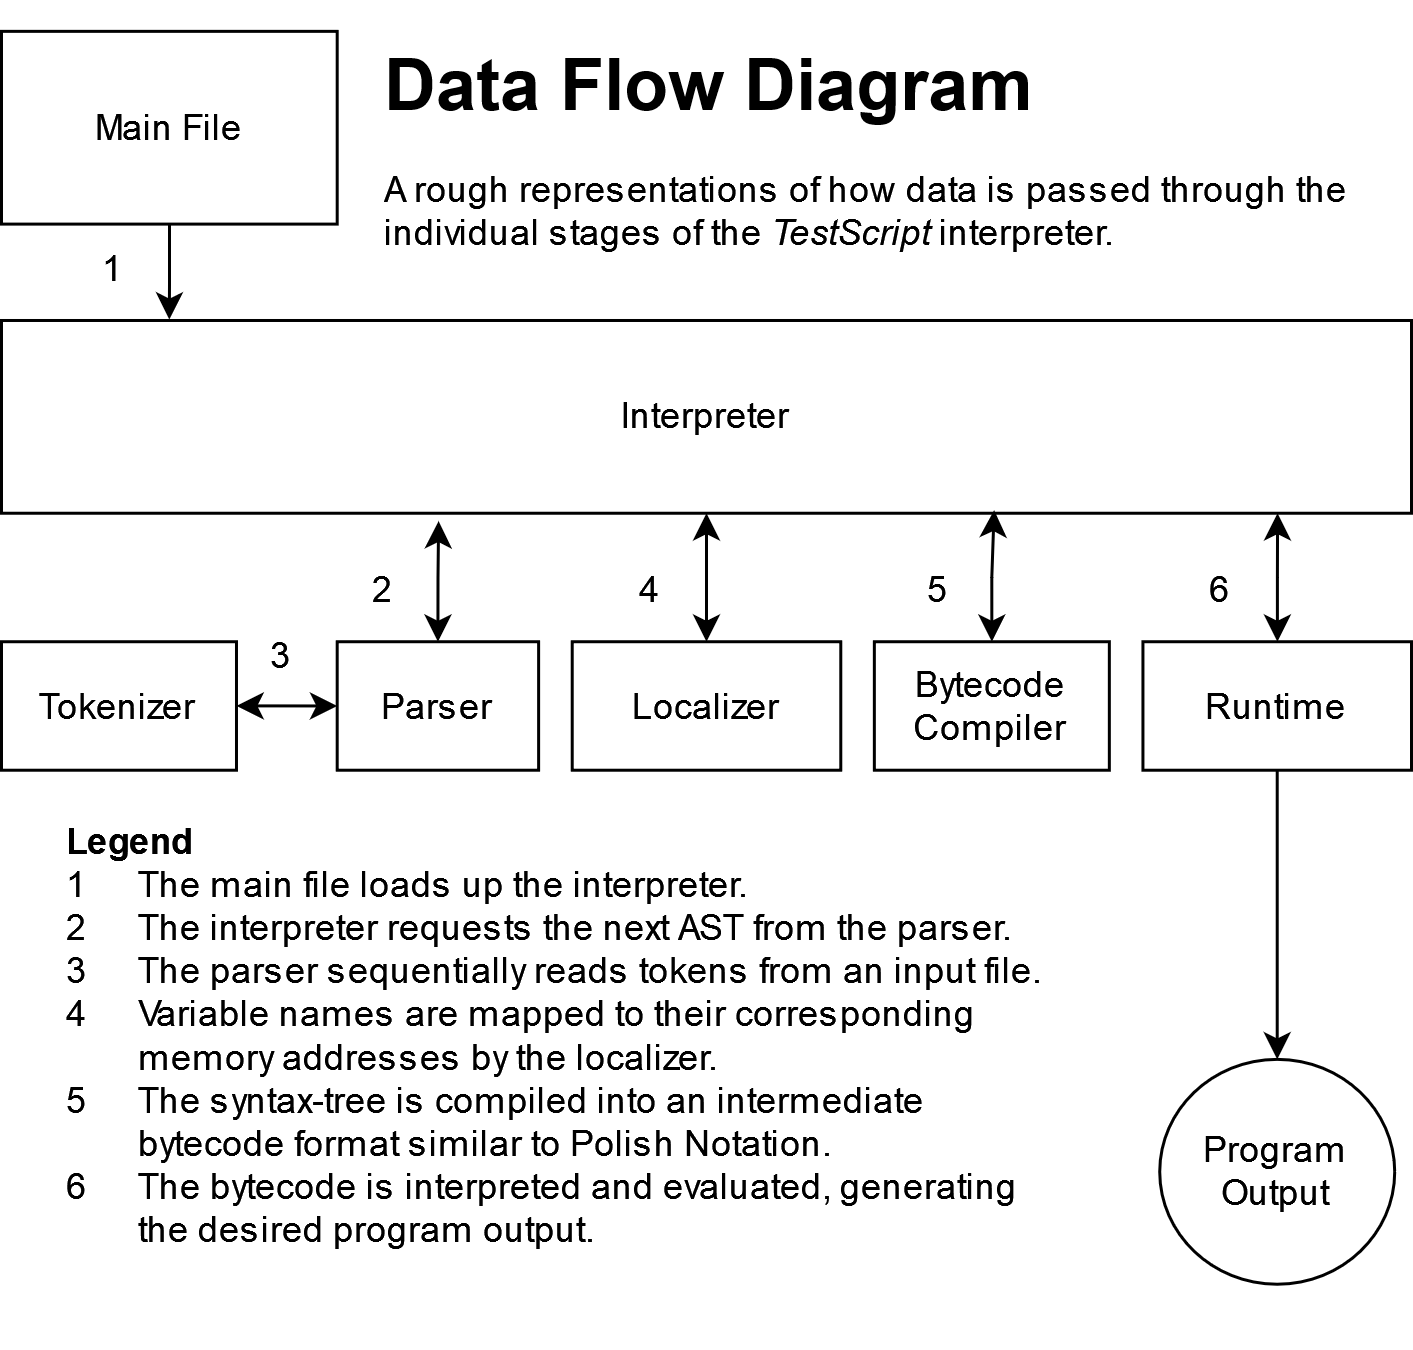
\includegraphics[width=0.6\textwidth]{paper/Data Flow Diagram.png}
    \caption{A \name{} Data Flow Diagram}
    \label{f_diagram}
\end{figure}

The above figure is a representation of how different components of the entire
\name{} implementation interact and work together. Each next stage performs
operations on the output data of the proper. The src/interpreter/interpreter.c
file, here depicted as 'Interpreter', chains all stages together.

\subsection{Implementing \name{}}
This section will explain the process of constructing and the inner workings of
the \name{} interpreter. It is therefore the most complicated and detailed section
in this paper. Examples will be made with both pseudo code and actual source
code from the project to further illustrate the decisions made during
interpreter design. The file paths used are relative to the project's root directory.

The syntax of \name{} is not specified in a formal programming language grammar,
but rather implemented from scratch in the files src/interpreter/tokenizer.c 
and src/interpreter/parser.c.

\subsubsection{The Entry-Point}
The entry point of the project lies in the src/main.c file.
The file implements the C main function, which is the entry-point of any
C application in general. Since the file is so small, here is its source code:
\code{src/main.c}{1}{999}

For the readers who do not know how to read source code, C in particular, here is a short
explanation of the basic syntax of the C language based on the src/main.c file:
\begin{itemize}
    \item \emph{Preprocessor Instructions.} Lines beginning with hashtags are
        C preprocessor instructions, they are dealt with by the C preprocessor.
        Preprocessing is what the compiler does before actually compiling the
        code.

        The most common preprocessor instructions are the following.
        On one hand there is \expr{\#include <header.h>}
        to include various definitions from a header file, i.e. to paste
        its content at where the 'include' statement lies.
        On the other hand exists \expr{\#define A B} used to
        define A as an alias for B and replace every following occurrence of A
        with B.

    \item \emph{Functions.} Functions in C are defined the following way:
        \expr{<return type> <function name>([arguments]) { <function body> }}
        or with a concrete, working example:
        \expr{int myFunction(int *arg) \{ printf("arg: \%p, arg); \}.}
        In main.c there is one function. The function's name is 'main', its
        return type is 'int', it has two arguments 'argc' and 'argv' and a
        function body containing what the function does.

    \item \emph{Pointers.} Pointers are variables that store memory addresses
        of data. In C-like syntax they are defined with the star (*) symbol.
        An example from src/main.c is 'FILE *input;'. That means that input is not
        actually a FILE, but rather the memory address to where a FILE is.

        To dereference the pointer, i.e. to actually retrieve the value stored
        at the memory address it contains, another star could be used as such:
        'FILE value = *input;'.
\end{itemize}

For those who are further interested in the C programming language, there are
many internet articles or tutorials about reading and understanding or
writing and compiling C code. One such example is the article 'The C Beginner's
Handbook' provided by freeCodeCamp.org linked in the sources\cte{freeCodeCamp}
on page \pageref{bibliography}.

Here is a very quick summary of what happens in the src/main.c file: the src/interpreter/interpreter.h
header file is included. In the main function, the program decides to either
read a program from the standard input or from a file. Then, the interpret function
from the said included header is called with the selected input.

\subsubsection{The Interpreter}
This section deals with the file src/interpreter/interpreter.c which guides
input data through the various stages of the \name{} interpreter in its
function 'interpret', which is called from the program's main function.

The 'interpret' function calls the parser to generate a syntax-tree from tokens retrieved
from the tokenizer implemented in src/interpreter/parser.c and 
src/interpreter/tokenizer.c respectively.

After that, variables with names are 'localized', meaning their names are
mapped to addresses in memory where their value is stored. Doing this before
bytecode compilation has a performance benefit. 
The mapping is done with a custom hashtable datastructure with average time
complexity of O(log n), n being the amount of different variables.

The syntax tree could now be interpreted directly, but as said, is instead converted
to an intermediate internal bytecode format by src/interpreter/bytecode.c.
This step is done so that code that is run multiple times does not convey
the problem of time overhead when traversing the syntax tree, but the current
implementation does not take advantage of this.

The final step is to process or execute said bytecode. This step is performed
by src/interpreter/runtime.c.

\subsubsection{The Tokenizer}
The tokenizer is implemented in src/interpreter/tokenizer.c. Its job is to
take source code in plain-text format as input and output so-called tokens.
These tokens represent groups of characters that belong together. In this paper's
implementation, each token has a strict type and a text content.
The different types of tokens and other things are defined in the header file
src/interpreter/tokenizer.h.

Here is an example of tokenization:
An input of 'std.test==23.4' would result in the following tokens according
to the tokenizer implementation of this paper:
\begin{enumerate}
    \item Token of type FIELD with content 'std.text'.
    \item Token of type SYMBOL with content '=='.
    \item Token of type NUMBER with content '23.4'.
\end{enumerate}
FIELD type tokens are later replaced by REFERENCE tokens during the stage of localization
and SYMBOL type tokens are mapped to EXPR by src/implementation/mappings/mapop.c
during parsing. NUMBER type tokens are replaced by an actual number type, which
is C's 'long double' type as specified in src/interpreter/bytecode.h.

The tokenizer used in this paper is a simple finite-state machine, reading
character by character and determining the token type as it goes.

These tokens are then directly consumed by the parser as described in the next
section.

\subsubsection{The Parser}
The parser, implemented in src/interpreter/parser.c, generates a syntax-tree
from tokens. The algorithm used is inspired by the Pratt Parsing\cte{pratt}
algorithm first described by Vaughan Pratt in 1973, which is a kind of precedence
parser based on recursive descent. There is a great simple explanation of the algorithm
by Jonathan Apodaca on dev.io\cte{devio} linked in the references on page 
\pageref{bibliography} which this paper's parser takes inspiration from.

The syntax tree in the implementation of \name{} consists of 'stnode' type
pointers, as defined in src/interpreter/parser.h. Each such node depending
on its 'nodetype', declared in src/interpreter/tokenizer.h,
is either a value-node storing a pointer to some data, e.g. a number or text, or a
parent-node referencing two child nodes and an operator, e.g. two numbers as
children and a plus-operator to signify an addition.

The difficult part of implementing a parser is precedence. Precedence and
associativity define the order of execution of statements. A simple example
would be to perform multiplication before addition, e.g. '2+3*4' would
result in 14 and is not the same as '(2+3)*4'. Therefore, each operator is
assigned a precedence, or priority, as well as an associativity, which is
either 'Left to Right' or 'Right to Left'. An example of associativity is
\emph{'20 / 10 / 2'}. Both in C as well as in \name{}, the division operator is
left-to-right associative, meaning the stated expression is the same as
\emph{'(20 / 10) / 2'} and not as \emph{'20 / (10 / 2)'}. Both precedence 
and associativity are properties that are defined in the file mapop.gpref for
each operator.

The parser implementation in src/interpreter/parser.c may be difficult to
read and understand, which is why the most important functions are explained here:
\begin{itemize}
    \item \emph{advance.} This function reads a new token from the tokenizer.
    \item \emph{secondary.} The 'secondary' function deals with parsing single,
        simple values that make up the start of an expression, such as numbers,
        fields, strings and it handles brackets, such as indexing with square
        brackets, functions or code blocks with curly braces and sub-expressions
        in standard brackets.
    \item \emph{expr.} The 'expr' function calls 'secondary' which acts
        as the basis for a new expression. It then repeatedly checks
        if an operator follows the secondary token and creates a tree of
        EXPR type stnodes, each having children which are recursively parsed
        and information about the operator.
    \item \emph{parse.} The parse function is a small wrapper which only
        calls the 'expr' function, initiating the parsing process.
\end{itemize}

Following is a piece of pseudocode to better illustrate the inner workings of the
parser which is based on a Pratt-parser. 
This is only an example and not completely accurate to the actual parser used
by this project.
% TODO: validate code
\code{pseudocode/parser.c}{1}{999}

\subsubsection{The Bytecode Compiler}
The bytecode compiler is part of the interpreter. Its job is to create a list
of byte-sized instructions and data from the syntax-tree the parser created.
Having such an intermediary bytecode format, instead of directly interpreting
the parse-tree can be beneficial. This is the case when the same piece of code
has to be run several times. Instead of generating a time and memory overhead 
having to walk along tree-nodes recursively, only the list of instructions in
the bytecode can be traversed, which is much faster. 

Not to be confused with machine-native bytecode, the bytecode compiler in \name{}
generates byte-sequences in an internal format, that are then interpreted. A
JIT compiler would instead compile the AST down to machine-native bytecode, which
could run directly on the system's hardware and would not have to be interpreted.

To generate such a sequence of bytes, \name{} recursively reads through the
binary tree created by the parser and pushes found instructions onto a stack,
which is in this case used similarly to a variable-sized list.
The algorithm used is inspired by Edsger Dijkstra's 'Shunting yard 
algorithm'\cte{shunting_yard}, traversing the tree post-order to create
a prefix notation. 

A prefix notation is a way to write down mathematical expressions, except
operators precede their operands, in contrast to the more common infix notation,
where operands surround the operator.

In src/interpreter/bytecode.c we can see, that first, the left operand and then
the right operand are added onto the stack of bytecode. Therefore, when
popping from the stack and evaluating instructions, the operands will have to
be read in reverse.
Here is an example:
\begin{enumerate}
    \item Assume the following mathematical expression in infix notation:
        \expr{\emph{'1 - 2 * 4 / (5 + 6)'}}
    \item In common prefix notation, also called Polish notation, the
        operators would now precede the operands as such:
        \expr{\emph{'- 1 (/ (* 2 4) (+ 5 6))'}}
    \item But in \name{} the operands are pushed onto the stack is reverse order.
        This would look like the following:
        \expr{\emph{'- (/ (+ 6 5) (* 4 2)) 1'}}
    \item The brackets are not needed, because for every operator, the amount
        of operands is known. This is the case as e.g. the subtraction operator
        and the negative operator, which are both a minus sign, are distinguished
        beforehand. This means the above statement would look like this:
        \expr{\emph{'- / + 6 5 * 4 2 1'}}
        This is an ideal abstraction of how data 
        is represented internally in \name{}.
\end{enumerate}

\subsubsection{The Runtime}
This is the last stage of interpreting program code as implemented in \name{}.
The runtime steps through the intermediary bytecode created by the bytecode
compiler and evaluates expressions by plugging in the provided values.
All available expressions are implemented in 
src/interpreter/processing/implementations.c.

The evaluation of expressions also works in a recursive manner. Here is an 
example of \name{}'s bytecode notation and how it would be evaluated at runtime:
\begin{itemize}
    \item Assume the input in \name{}'s bytecode to resemble the following expression: 
        \expr{\emph{'- 6 * 3 4'}}
        In infix notation, this would be equivalent to 
        \expr{\emph{'(4 * 3) - 6'}.}
    \item The runtime will read through the bytecode left-to-right. First it will
        notice the subtraction-operator and accordingly assume that two
        operands must follow.
    \item The processing function will call itsself
        and notice the 6, a number, and therefore a value. The function simply returns the 6
        to the subtraction expression. This 6 will be the right-hand operator
        of the subtraction.
    \item The subtraction will then call the processing function again to find
        the left operand. As the processing function reads a multiplication operator,
        it now recursively reads through that expression's right and then left
        operator, which would be 3 and for respectively and compute and return
        the result of the multiplication, which is 12.
    \item Now the subtraction knows its right- and left-hand operators, 6 and 12,
        and again, calculate and return the result, which is 6.
\end{itemize}

That is it. With all the expressions available, entire programs
can now be interpreted.

\section{Results}

% TODO: add examples in /examples/
\name{} is built upon the implementation of a recursive Pratt
parser and a basic tokenizer. Most actual features are reliant upon this
foundation, such as operators and the standard library built into \name{}.

\subsection{Syntax}
The syntax of \name{} can be compared to the syntax of JavaScript, except
there are no keywords at all, and everything is controlled via operators,
which are non-alphanumeric characters. Such operators include the plus-sign 
for addition, or the equals-sign for variable assignment.

Following is a piece of example \name{} code, printing out the first ten numbers
of the fibonacci sequence, as well as a disection of how that same code is interpreted.
\code{examples/fibonacci.nts}{1}{999}
\begin{itemize}
\item The source code begins by declaring two variables \emph{a} and \emph{b}, which
    will be utilized to keep track of the data used to calculate fibonacci numbers.
    The memory allocation is done by creating a tuple of \emph{a} and \emph{b}, as suggested by 
    the comma seperating the two. Since both variables \emph{a} and \emph{b} are not yet
    known to the interpreter, they are automatically created and assigned a value
    which has no content and the \emph{undefined} typing.
\item The two variables \emph{a} and \emph{b} are then reassigned new values on line
    2 of the program. In this case it is numbers with values zero and one respectively.
    In this example, the two expressions are seperated by a space, but they can
    also be separated by newline-characters or semicolons.
\item Another variable \emph{count} is declared and defined as number in one step on line 4.
    This variable will be used to limit the amount of numbers the program outputs.
\item Yet another variable, \emph{f}, is declared and assigned a function as its
    value on line 6. In \name{}, normal functions do not have any arguments, 
    but they can interact with variables that were created outside their scope.
\item Lines 7 to 10 hold mathematical expressions. At first, a is assigned its current value
    plus the current value of b. Then in line 8, b is assigned the now new value of a minus the
    current value of b, which corresponds to the value of a before it was just reassigned.
    Lastly the variable \emph{count} is decremented by one.
\item Now come the interesting parts of this program.
    On lines 12 and 13, the function \emph{std.print} is referenced. This function is implemented
    in plain C code, which internally is not handled the same as regular functions in \name{},
    and is wrapper to C's function \emph{printf}. The \emph{std.print} function
    takes any \name{} variable or value and prints it to standard output. On line 13, the "\\n"
    is replaced by a newline-character, as \name{} can interpret Java-like escape-sequences.
\item Another standard-library function is \emph{std.if}. It takes two or three arguments.
    If the first argument is true, then the second, else the the third argument or 
    \emph{undefined} is returned. A value is true, only if it is a number not equal to zero
    or a non-empty string. In the case of this example, \emph{std.if} returns \emph{f} if 
    count is greater than zero, and an empty function if count reaches zero. The two
    brackets following the call of the \emph{std.if} function signal yet another call to the
    returned value.
\item The final thing left to do is to get the ball roling by calling the function \emph{f} for
    the first time. As stated above, it will now print numbers and recursively call itsself,
    until the variable \emph{count} reaches a value of zero.
\end{itemize}

\subsection{Name Shadowing}
Here is another example, which in contrast to the example above, focuses on a
security concept implemented in \name{}.
\code{examples/exec.nts}{1}{999}
The code begins by creating the variable \emph{var}, which holds a string, and
\emph{f}, which calls the function \emph{std.exec} with var as argument.
Line number six holds a comment, indicated by the two slashes at the start of the line.
Comments are ignored by the \name{} interpreter and their purpose is to contain notes
and explanations inside the source code itself. Another type of commends are block-comments
which span across multiple lines, such as on lines 9 to 12.
On line seven, the \emph{std.exec} function is called for the first time. It runs the
command it is given as argument in the user's shell, which is most commonly \emph{cmd} on
Microsoft Windows and \emph{bash} on most Linux distributions. In this example, \emph{std.exec}
launches the Firefox browser, but it is capable of all kinds of things that can otherwise be
done in the shell, such as delete files or shut down the computer.

That is why in most cases, the \emph{std.exec} function can be a risk waiting to be exploited
by malicious \name{} programs. To solve this problem, there is the hashtag-operator, whose purpose
it is to delete access to a variable through the specified name. It is used on line 13 of the
example to remove access to the \emph{std.exec} function, which is why the call to that function
on line 16, trying to shut down the computer, will result in an error. Unexpectedly though, the
call on line 20 to the function \emph{f} which was created as an as to \emph{std.exec} will work.

This security concept enforces the use of a top-down programming model. First, safe-to-use aliases
to dangerous functions have to be created. Then, access to all those exploitable functions is
revoked. This way, running unknown code can only access data and functions that are being provided.
This contrasts the models of languages like Python. In Python, each seperate source file can
make use of the \emph{import} keyword to include other files. Files imported this way do not
have access or knowledge about the variables that exist in the file that includes them.
In \name{}, each imported file would instead have access to all variables and functions that
are made available to it, instead of having to include or import them seperately.
This leads to another problem, but that is what the next section will be all about.

\section{Discussion}

\subsection{Distribution}
% TODO

\subsection{Limitations}
\name{} is a programming language without a doubt. But it is not perfect in any
way. There are limitations that make it practically unusable for actual
professional projects. In this section, a few shortcomings of \name{} are listed
and reasoned over.

\subsubsection{Numbers}
% TODO

\subsubsection{Memory Leaks}
Memory leaks happen, when a program reserves memory to store some data, but
never frees up the space for use for other programs, even though the data
has long been discarded and is of no further use.
In \name{}, memory leaks are a major problem. Even though barely noticable for small
programs it interprets, \name{} does not have proper setups in place to free up
all used memory that is not used any longer.

Other programming languages, notably object-oriented languages such as Java,
use Garbage-Collection, which automatically tracks unused allocated memory and
frees it up automaticadlly. While this is also the case with \name{}, there are
many internal flaws that have nothing to do with variables used in a \name{}
program, but rather internally. 

A major reason for the memory leaks, but not an excuse, is the nature of the
C programming language the \name{} interpreter was written in. The C language and
compiler do not keep track of states in which certain blocks of memory are
forgotten about and warn the developer, instead, memory leaks happen.
More modern C alternatives such as Rust have a ownership-system in place,
in which any allocated memory has a function as an owner, and when the function
is done processing, the memory is automatically freed. Such systems are a
helpful tool for developers to create better programs with low mental overhead,
and are what programming language design should be all about.

\subsubsection{Single-Threaded}
The \name{} interpreter does not implement any multi-threaded, meaning parallel
running, programs as most other languages do. Instead, any \name{} program can
only be interpreted and run sequentially. Since most modern computer processors
are equipped with a handful of processing cores and threads, not being able to
make use of those is a major downside and in itsself a reason not to use this
language.

\subsubsection{Lack of a Development Environment}
This is certainly the greatest problem of \name{}, aside the countless smaller
bothering aspects.

Most modern programming languages do not only consist
of a language specification and a compiler or interpreter, but of many more
tools surrounding them.
Such tools can include a package-manager, with which people around the world
can share code. Examples would be npm\cte{npm} or cargo\cte{cargo}, 
the 'Node Package Manager' for JavaScript applications and and Rust's package 
manager respectively.

\subsection{Interesting Ideas untouched}
Creating the ideal programming language takes a lot of planning and sketching
out. This section of the paper gives insight on interesting ideas or concepts
that are great to have and are used in other programming languages, but not 
could not be implemented into \name{}.

\subsubsection{Foreign Function Interfaces}
A foreign function interface\cte{FFI} often abbreviated as FFI,
is a mechanism by which one programming language can call functions written 
in another. This makes a language more attractive, as it can be used with
existing libraries from another language, instead of functions having to be
re-written. Enabling C function calls often allows a certain language to
directly interact with system libraries or the operating system itsself.

Foreign function interfaces are available in many modern languages.
Examples are Java, Python and Rust.
Java enables users to call C, C++ and even assembly code with the Java Native
Interface\cte{JNI}, JNI for short, whereas within Python C function can
be run with the standard ctypes\cte{ctypes} library.

Foreign function interfaces are specially difficult to implement, or implement
right. Let us assume a programming language interpreter \name{} written in C that
would like to call some functions that are part of yet another C program or
library. The problem lies in the fact that at runtime, C does not know
structure of the functions to be called, say return- or argument-types, which
is by the way where the term foreign functions originates from. This is why the
\name{} developer would have to provide that information by re-declaring the
function inside \name{}, so that, with some trickery, data can be passed to and
received from the function in the correct format, preventing a segmentation
fault. The libffi\cte{libffi} C-library, which is also used by Java and
Python for this purpose, can be used to load and call such foreign functions.

\subsubsection{Reflection}
Reflection\cte{reflection}, also called reflective programming, describes
the ability of a program to examine and modify its own structure and behavior 
at runtime. An example would be self-modifying code. This can easily be
achieved in assembly language, which inherently does not differentiate between
data and instructions.
Another example is Java, providing methods and classes in the java.lang.reflect
package that enable developers to examine and change properties or functions
of objects.
The advantage of reflection over not having it is that it allows for non-static
programs and program flows, effectively making smaller executables and more
resource efficient programs, as those programs can adjust themselves to run
differently under different conditions at runtime.
The easiest and simplest way to go about implementing Reflection in \name{} is
certainly to allow the interpretation of strings at runtime. That way, strings
holding program instructions can be created and modified and later executed.

\section{Index}
\section{Closing Words}
\section{Declaration of Autonomy}
Hereby I, Florian Donnelly, declare to have written this paper, also including
the entire source code of \name{} by myself using resources listed under the
'references' section on page \pageref{bibliography}.

\newpage\section{Bibliography}
\pagelabel{bibliography}\printbibliography[heading=none]

\section{List of Figures}\listoffigures
\vspace{1cm}
Figure \ref{f_mandelbrot} was generated using a \name{} program, the source code
can be found in the file examples/mandelbrot.nts.
Figure \ref{f_diagram} was created using an online diagram creation tool available
on app.diagrams.net \cte{drawio}.

% TODO: check correctness of all file paths!! e.g. src/...

\newpage\section{Appendix}
The appendix contains the complete source code of \name{}.

% Append all soruce files
% \foreach \f in \files{\pagelabel{\f}\code{\f}{1}{9999}}

\end{document}

